\documentclass[a4paper, 12pt]{article}

% NOTE: packates que se usaran en todo el proyecto
% paquetes para el idioma
\usepackage[T1]{fontenc}
\usepackage[spanish]{babel}
\defineshorthand{"-}{\babelhyphen{hard}} % para que los guiones o dashes no se fusionen

\usepackage[utf8]{inputenc}

\usepackage[top=25mm, left=25mm, bottom=25mm, right=18mm, headheight=25mm, b5paper]{geometry}

\usepackage{graphicx} % Imagenes
\usepackage{parskip} % Arreglo de la tabulación en el documento
\usepackage{xcolor, soul} % Para poder usar colores
\usepackage{titletoc} % Para personalizar la tabla de contenido
\usepackage{titlesec} % Para personalizar los títulos de los capítulos y las secciones
\usepackage{textcomp} % Agrega el paquete textcomp en el preámbulo
\usepackage{fancyhdr} % Para trabajar con el encabezado
\usepackage{amssymb} % Agrega el paquete amssymb en el preámbulo
\usepackage{listings} % Para usar el paquete listings y sintaxis de códigos
\usepackage{lipsum} % para generar texto aleatorio
\usepackage{booktabs} % Para usar tablas personalizadas.
\usepackage{lmodern} % Latin moderno
 % packages

\graphicspath{{./assets/}}

\begin{document}

\begin{flushright}
  Por: \textit{Jesús Gabriel Rivera}

  En \faGithub \hspace{0.1cm} Github como \lineCode{\textit{grChad}}

  Me he basado en el repositorio de \faGithub \lineCode{\textit{andersontr15/clean-code-javascript-es}}
\end{flushright}

\hrulefill % Línea horizontal
\vspace{0.5cm} % space

\begin{center}
  \huge\textbf{\textblue{Clean Code}} \textjs{JavasCript}
	\vspace{0.5cm} % space
\end{center}

\section{Introducción}

\begin{center}
  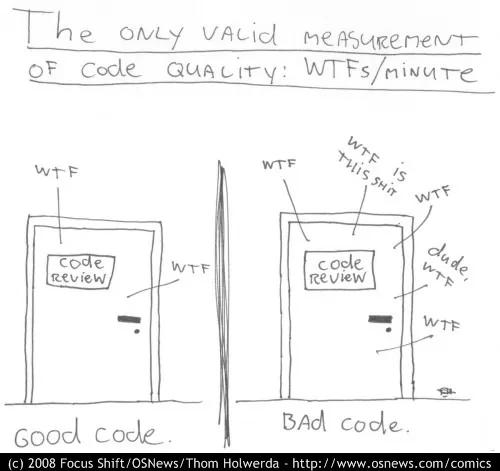
\includegraphics[width=11cm]{introduction_bad_code} % Logo de Lua
	\vspace{0.5cm} % space
\end{center}

Los principios de la ingeniería de software, del libro de Robert C. Martin \textblue{\textit{Clean Code}}, adaptado para JavasCript. Esta no es una guía de estilo, en cambio, es una guía para crear software que sea reutilizable, comprensible y que se pueda mejorar con el tiempo.

No hay que seguir tan estrictamente todos los principios en este libro, y vale la pena mencionar que hacia muchos de ellos habrá controversia en cuanto al consentimiento. Estas son reflexiones hechas después de muchos años de experiencia colectiva de los autores de \textit{Clean Code}.

Una cosa más: saber esto no te hará un mejor ingeniero inmediatamente, y tampoco trabajar con estas herramientas durante muchos años garantiza que nunca te equivocarás. Cualquier código empieza primero como un borrador, como arcilla mojada moldeándose en su forma final. Por último, arreglamos las imperfecciones cuando lo repasamos con nuestros compañeros de trabajo. No seas tan duro contigo mismo por los borradores iniciales que aún necesitan mejorar. ¡Trabaja más duro para mejorar el programa!
 % section 01: 'Introducción'
\newpage

\newpage % saltar a la siguiente pagina

\section{Dibujando formas con canvas}

Ahora que hemos preparado nuestro entorno \code{canvas}, podemos entrar en detalles de cómo dibujar en el \code{canvas}. Al final de esta sección, habrás aprendido cómo dibujar rectángulos, triángulos, líneas, arcos y curvas, familiarizándote con algunas de las formas básicas. Trabajar con trazados es esencial a la hora de dibujar objetos en el \code{canvas} y veremos cómo hacerlo.

\subsection{La cuadrícula}

Antes de empezar a dibujar, tenemos que hablar de la cuadrícula del \code{canvas} o del espacio de coordenadas. Nuestra estructura \texthtml{HTML} de la sección anterior tenía un elemento de \code{canvas} de 150 pixels de ancho y 150 pixels de alto.

\vspace{0.5cm} % separación vertical
\begin{center}
	\begin{tikzpicture}
		\draw[color=gray, help lines, dashed] (0,0) grid (6.5,-6.5);
		\draw[color=gray] (0,0) rectangle (6.5,-6.5); % Cuadrado de esquina (0,0) a (2,2)
		\node[color=black, rotate=90, yshift=-10pt] at (6.5,-3) {$Height$};
		\node[color=black, yshift=-10pt] at (3.3,-6.5) {$Width$};

		% Ejes x e y
		\draw[color=black, very thick] (-0.2,0) -- (7,0) node[right] {$x$};
		\draw[color=black, very thick] (0,0.2) -- (0,-7) node[left] {$y$};

		% flechas
		\draw[color=black] (7,0) to (6.9, 0.1);
		\draw[color=black] (7,0) to (6.9, -0.1);
		\draw[color=black] (0, -7) to (0.1, -6.9);
		\draw[color=black] (0, -7) to (-0.1, -6.9);

		% Marcar el origen (0,0)
		\filldraw[color=black] (0,0) circle (2pt) node[anchor=north east, yshift=20pt] {$(0,0)$};

		% Flechas indicando la posición del punto (5, -5)
		\draw[color=blue] (2.5,0) -- (2.5,-2.5);
		\draw[color=blue] (0,-2.5) -- (2.5,-2.5);

		% Etiquetar los ejes de punto (2.5, -2.5)
		\node[color=blue, above right] at (1,-2.5) {$x$};
		\node[color=blue, above left] at (2.5,-1.5) {$y$};

		% Dibujar un cuadrado con color
		\fill[color=teal] (2.5, -2.5) rectangle (5.5, -5.5);
		\filldraw[color=blue] (2.5,-2.5) circle (1pt);

		% Marcar el punto (2.5, -2.5)
	\end{tikzpicture}
\end{center}
\vspace{0.5cm} % separación vertical


Normalmente, 1 unidad en la cuadrícula corresponde a 1 pixel en el canvas. El origen de esta cuadrícula se sitúa en la esquina superior izquierda en la \lineCode{coordenada (0,0)}. Todos los elementos se colocan en relación con este origen. Así que la posición de la esquina superior izquierda del cuadrado azul se sitúa a \code{X} pixels de la izquierda y a \code{Y} pixels de la parte superior, en la coordenada \code{(x,y)}. Más adelante en esta sección veremos cómo podemos trasladar el origen a una posición diferente, rotar la cuadrícula e incluso escalarla, pero por ahora nos ceñiremos a la posición por defecto.

\subsection{Dibujar rectángulos}

A diferencia de \textblue{SVG}, \taghtml{\textless canvas\textgreater} sólo admite dos formas primitivas: rectángulos y trazados (listas de puntos conectados por líneas). Todas las demás formas deben crearse combinando uno o más trazados. Por suerte, tenemos un surtido de funciones de dibujo de trazados que hacen posible componer formas muy complejas.

Primero veamos el \code{rectángulo}. Hay tres funciones que dibujan rectángulos en el canvas:

\vspace{0.5cm} % separación vertical
\begin{lstlisting}[language=TypeScript, style=mystyle]
  // (1) Dibuja un rectangulo relleno.
  fillRect(x, y, width, height)
\end{lstlisting}

\newpage % saltar a la siguiente pagina


\begin{lstlisting}[language=TypeScript, style=mystyle]
  // (2) Dibuja un contorno rectangular.
  strokeRect(x, y, width, height) (en-US)
\end{lstlisting}

\begin{lstlisting}[language=TypeScript, style=mystyle]
  // (3) Borra el area rectangular especificada, haciendola totalmente transparente.
  clearRect(x, y, width, height)
\end{lstlisting}
\vspace{0.5cm} % separación vertical

Cada una de estas tres funciones toma los mismos parámetros. \textblue{x} y \textblue{y} especifican la posición en el \code{canvas} (relativa al origen) de la esquina superior izquierda del rectángulo. \code{width} y \code{height} proporcionan el tamaño del rectángulo.

A continuación se muestra la función \code{draw()} de la página anterior, pero ahora hace uso de estas tres funciones.

\subsubsection*{Ejemplo de forma rectangular:}

\begin{lstlisting}[language=TypeScript, style=mystyle]
  function draw() {
    const canvas = document.getElementById("canvas");
    if (canvas.getContext) {
      const ctx = canvas.getContext("2d");

      ctx.fillRect(25, 25, 100, 100);
      ctx.clearRect(45, 45, 60, 60);
      ctx.strokeRect(50, 50, 50, 50);
    }
  }
\end{lstlisting}
\vspace{0.5cm} % separación vertical

La salida de este ejemplo seria este:

\vspace{0.5cm} % separación vertical
\begin{center}
	\begin{tikzpicture}
		\fill[black] (0, 0) rectangle (5, -5); % rectángulo negro
		\filldraw[white] (1, -1) rectangle (4, -4); % rectángulo blanco
		\draw[black] (1.3, -1.3) rectangle (3.7, -3.7); % rectángulo negro
	\end{tikzpicture}
\end{center}
\vspace{0.5cm} % separación vertical

La función \code{fillRect()} dibuja un gran cuadrado negro de 100 pixels en cada lado. La función \code{clearRect()} borra un cuadrado de 60x60 pixels del centro, y luego se llama a \code{strokeRect()} para crear un contorno rectangular de 50x50 pixels dentro del cuadrado borrado.

En las próximas páginas veremos dos métodos alternativos para \code{clearRect()}, y también veremos cómo cambiar el color y el estilo de trazo de las formas renderizadas.

A diferencia de las funciones de trazado que veremos en la siguiente sub-sección, las tres funciones de rectángulo dibujan inmediatamente en el canvas.

\newpage % saltar a la siguiente pagina
\subsection{Dibujando paths}

Veamos ahora los \code{paths}(trazos). Un \code{paths} es una lista de puntos, conectados por segmentos de líneas que pueden ser de diferentes formas, curvas o no; de diferente anchura y de diferente color. Un \code{path}, o incluso un sub-path, puede ser cerrado. Para hacer formas usando trazos, damos algunos pasos adicionales:

\begin{enumerate}
	\item Primero, se crea el path o trazo.
	\item Luego, se utiliza comandos de dibujo para dibujar en el path.
	\item Una vez creado el path, puedes trazar o rellenar el path para renderizarlo.
\end{enumerate}

\vspace{0.5cm} % separación vertical
Aquí están las funciones utilizadas para realizar estos pasos:

\begin{description}
	\listCustom{beginPath():} Crea un nuevo trazado. Una vez creado, los futuros comandos de dibujo se dirigen al trazado y se utilizan para construirlo.
	\listCustom{Métodos de path:} Métodos para establecer diferentes paths para los objetos.
	\listCustom{closePath():} Añade una línea recta al path, que va al inicio del sub-path actual.
	\listCustom{stroke():} Dibuja la forma trazando su contorno.
	\listCustom{fill():} Dibuja una forma sólida rellenando el área de contenido del trazo.
\end{description}

\vspace{0.5cm} % separación vertical
El primer paso para crear un trazo(\code{path}) es llamar a \code{beginPath()}. Internamente, los trazos se almacenan como una lista de sub-trazos (líneas, arcos, etc.) que juntos forman una forma. Cada vez que se llama a este método, la lista se restablece y podemos empezar a dibujar nuevas formas.

\vspace{0.5cm} % separación vertical
\begin{tcolorbox}
	[colback=red!5!white,colframe=cyan,fonttitle=\bfseries,title={\faLightbulbO\, Nota:}]

	Cuando el trazo actual está vacío, como por ejemplo inmediatamente después de llamar a \code{beginPath()}, o en un canvas recién creado, el primer comando de construcción del trazo siempre se trata como un \code{moveTo()}, independientemente de lo que realmente sea. Por esta razón, casi siempre querrá establecer específicamente su posición inicial después de reiniciar un trazo.
\end{tcolorbox}
\vspace{0.5cm} % separación vertical

El segundo paso es llamar a los métodos que realmente especifican los trazos a dibujar. Los veremos en breve.

El tercer paso, y opcional, es llamar a \code{closePath()}. Este método intenta cerrar la forma dibujando una línea recta desde el punto actual hasta el inicio. Si la forma ya ha sido cerrada o sólo hay un punto en la lista, esta función no hace nada.

\vspace{0.5cm} % separación vertical
\begin{tcolorbox}
	[colback=red!5!white,colframe=cyan,fonttitle=\bfseries,title={\faLightbulbO\, Nota:}]

	Cuando se llama a \code{fill()}, cualquier forma abierta se cierra automáticamente, por lo que no es necesario llamar a \code{closePath()}. Este no es el caso cuando se llama a \code{stroke()}.
\end{tcolorbox}
\vspace{0.5cm} % separación vertical

\newpage % saltar a la siguiente pagina
\subsubsection{Dibujar un triángulo}
Por ejemplo, el código para dibujar un triángulo sería algo así:

\vspace{0.5cm} % separación vertical
\begin{lstlisting}[language=TypeScript, style=mystyle]
  function draw() {
    const canvas = document.getElementById("canvas");
    if (canvas.getContext) {
      const ctx = canvas.getContext("2d");

      ctx.beginPath();
      ctx.moveTo(75, 50);
      ctx.lineTo(100, 75);
      ctx.lineTo(100, 25);
      ctx.fill();
    }
  }
\end{lstlisting}
\vspace{0.5cm} % separación vertical

El resultado se ve así:

\begin{center}
	\begin{tikzpicture}
		\fill[black] (0,-2) -- (2,0) -- (2,-4) -- cycle;
	\end{tikzpicture}
\end{center}
\vspace{0.5cm} % separación vertical

\subsubsection{Dibujando con el lápiz}
Una función muy útil, que en realidad no dibuja nada sino que se convierte en parte de la lista de trazos descrita anteriormente, es la función \code{moveTo()}. La mejor manera de pensar en esto es como \textblue{levantar un bolígrafo o un lápiz} de un lugar en un pedazo de papel y colocarlo en el siguiente.

\begin{description}
	\listCustom{moveTo(x, y):} Muévete como usando el lápiz, por las coordenadas \textblue{x} e \textblue{y}.
\end{description}
\vspace{0.5cm} % separación vertical

Cuando se inicializa el canvas o se llama a \code{beginPath()}, normalmente se querrá utilizar la función \code{moveTo()} para colocar el punto de partida en otro lugar. También podemos usar \code{moveTo()} para dibujar trazos no conectados. Echa un vistazo a la cara sonriente de abajo.

\newpage % saltar a la siguiente pagina
Para probarlo por ti mismo, puedes utilizar el siguiente fragmento de código. Sólo tienes que pegarlo en la función \code{draw()} que vimos antes.

\vspace{0.5cm} % separación vertical
\begin{lstlisting}[language=TypeScript, style=mystyle]
function draw() {
  const canvas = document.getElementById("canvas");
  if (canvas.getContext) {
    const ctx = canvas.getContext("2d");

    ctx.beginPath();
    ctx.arc(75, 75, 50, 0, Math.PI * 2, true); // Circulo externo
    ctx.moveTo(110, 75);
    ctx.arc(75, 75, 35, 0, Math.PI, false); // Boca (en el sentido de las agujas del reloj)
    ctx.moveTo(65, 65);
    ctx.arc(60, 65, 5, 0, Math.PI * 2, true); // Ojo izquierdo
    ctx.moveTo(95, 65);
    ctx.arc(90, 65, 5, 0, Math.PI * 2, true); // Ojo derecho
    ctx.stroke();
  }
}
\end{lstlisting}
\vspace{0.5cm} % separación vertical

El resultado se ve así:

\begin{center}
	\begin{tikzpicture}
		% Circulo con centro en (0,0), radio de 1
		\draw (0, 0) circle (2);

		% Arco: centro en (0, 0), angulo de 0 a 45 grados, radio de 2
		\draw (1.5, 0) arc (0: -180: 1.5);

		\draw (-0.6, 0.5) circle (0.2); % ojo izquierdo
		\draw (0.6, 0.5) circle (0.2); % ojo derecho
	\end{tikzpicture}
\end{center}
\vspace{0.5cm} % separación vertical

Si quisieras ver las líneas conectadas, puedes eliminar las líneas que llaman a \code{moveTo()}.

\subsubsection{Líneas}

Para dibujar líneas rectas, utilice el método \code{lineTo()}.

\begin{description}
	\listCustom{lineTo(x, y):} Dibuja una línea desde la posición actual de dibujo hasta la posición especificada por \textblue{x} e \textblue{y}.
\end{description}
\vspace{0.5cm} % separación vertical

Este método toma dos argumentos, \textblue{x} e \textblue{y}, que son las coordenadas del punto final de la línea. El punto de partida depende de los trazos anteriores, donde el punto final del trazo anterior es el punto de partida del siguiente, etc. El punto de partida también puede cambiarse utilizando el método \code{moveTo()}.

\newpage % saltar a la siguiente pagina
El ejemplo siguiente dibuja dos triángulos, uno relleno y otro contorneado.

\vspace{0.5cm} % separación vertical
\begin{lstlisting}[language=TypeScript, style=mystyle]
  function draw() {
    const canvas = document.getElementById("canvas");
    if (canvas.getContext) {
      const ctx = canvas.getContext("2d");

      // Triangulo relleno
      ctx.beginPath();
      ctx.moveTo(25, 25);
      ctx.lineTo(105, 25);
      ctx.lineTo(25, 105);
      ctx.fill();

      // Triangulo contorneado
      ctx.beginPath();
      ctx.moveTo(125, 125);
      ctx.lineTo(125, 45);
      ctx.lineTo(45, 125);
      ctx.closePath();
      ctx.stroke();
    }
  }
\end{lstlisting}
\vspace{0.5cm} % separación vertical

Esto comienza llamando a \code{beginPath()} para iniciar un nuevo trazo. A continuación, utilizamos el método \code{moveTo()} para mover el punto de partida a la posición deseada. Debajo de esto, se dibujan dos líneas que forman los dos lados del triángulo.

\vspace{0.5cm} % separación vertical
\begin{center}
	\begin{tikzpicture}
		% Triangulo relleno
		\fill[black] (0,0) -- (3,0) -- (0,-3) -- cycle;
		\draw (4, -1) -- (4, -4) -- (1, -4) -- cycle;
	\end{tikzpicture}
\end{center}
\vspace{0.5cm} % separación vertical

Notará la diferencia entre el triángulo relleno y el trazo. Esto se debe, como se ha mencionado anteriormente, a que las formas se cierran automáticamente cuando se rellena un trazo, pero no cuando se traza. Si omitimos el \code{closePath()} para el triángulo trazo, sólo se habrían dibujado dos líneas, no un triángulo completo.

\newpage % saltar a la siguiente pagina
\subsubsection{Arcos}

Para dibujar arcos o círculos, utilizamos los métodos \code{arc()} o \code{arcTo()}.

\begin{description}
	\listCustom{arc(x, y, radius, startAngle, endAngle, anticlockwise):} Dibuja un arco centrado en la \\ posición \code{(x, y)} con radio \code{r} que comienza en \code{startAngle} y termina en \code{endAngle} yendo en la dirección indicada por \code{counterclockwise} (por defecto en el sentido de las agujas del reloj).

	\listCustom{arcTo(x1, y1, x2, y2, radius):} Dibuja un arco con los puntos de control y el radio dados, conectado al punto anterior por una línea recta.
\end{description}
\vspace{0.5cm} % separación vertical

Veamos con más detalle el método \textblue{arc}, que toma seis parámetros: \textblue{x} e \textblue{y} son las coordenadas del centro del círculo sobre el que se dibujará el arco. El parámetro radio se explica por sí mismo. Los parámetros \code{startAngle} y \code{endAngle} definen los puntos inicial y final del arco en radianes, a lo largo de la curva del círculo. Se miden desde el \lineCode{eje x}. El parámetro \code{counterclockwise} es un valor \lineCode{Booleano} que, cuando es \code{true}, dibuja el arco en sentido contrario a las agujas del reloj; en caso contrario, el arco se dibuja en sentido de las agujas del reloj.

\vspace{0.5cm} % separación vertical
\begin{tcolorbox}
	[colback=red!5!white,colframe=cyan,fonttitle=\bfseries,title={\faLightbulbO\, Nota:}]

	Los ángulos en la función \code{arc()} se miden en radianes, no en grados. Para convertir los grados en radianes puedes utilizar la siguiente expresión de \textjs{JavaScript}:

	\vspace{0.5cm} % separación vertical
	\begin{center}
		\lineCode{ radianes = (Math.PI/180)*grados }
	\end{center}
\end{tcolorbox}
\vspace{0.5cm} % separación vertical

El siguiente ejemplo es un poco más complejo que los que hemos visto anteriormente. Dibuja 12 arcos diferentes, todos con diferentes ángulos y rellenos.

Los dos bucles \lineCode{\textbf{for}} son para recorrer las filas y columnas de arcos. Para cada arco, iniciamos un nuevo trazo llamando a \code{beginPath()}. En el código, cada uno de los parámetros del arco está en una variable para mayor claridad, pero no necesariamente se haría eso en la vida real.

Las coordenadas \textblue{x} e \textblue{y} deberían ser lo suficientemente claras. radius y \code{startAngle} son fijos. \code{endAngle} comienza en 180 grados (medio círculo) en la primera columna y se incrementa en pasos de 90 grados, culminando en un círculo completo en la última columna.

La sentencia para el parámetro \code{clockwise} hace que la primera y tercera fila se dibujen como arcos en el sentido de las agujas del reloj y la segunda y cuarta fila como arcos en sentido contrario. Por último, la sentencia \lineCode{\textbf{if}} hace que la mitad superior tenga arcos trazados y la mitad inferior arcos rellenos.

\vspace{0.5cm} % separación vertical
\begin{tcolorbox}
	[colback=red!5!white,colframe=cyan,fonttitle=\bfseries,title={\faLightbulbO\, Nota:}]

	Este ejemplo requiere un \code{canvas} ligeramente más grande que los otros de esta página:\\
	150 x 200 pixels.
\end{tcolorbox}
\vspace{0.5cm} % separación vertical

\newpage % nueva página
\begin{lstlisting}[language=TypeScript, style=mystyle]
  function draw() {
    const canvas = document.getElementById("canvas");
    if (canvas.getContext) {
      const ctx = canvas.getContext("2d");

      for (let i = 0; i < 4; i++) {
        for (let j = 0; j < 3; j++) {
          ctx.beginPath();
          const x = 25 + j * 50; // Coordenada x
          const y = 25 + i * 50; // Coordenada y
          const radius = 20; // Radio del Arco
          const startAngle = 0; // Punto inicial del Circulo
          const endAngle = Math.PI + (Math.PI * j) / 2; // Punto final del Circulo
          const counterclockwise = i % 2 !== 0; // En el sentido de las agujas del reloj o en sentido contrario

          ctx.arc(x, y, radius, startAngle, endAngle, counterclockwise);

          if (i > 1) {
            ctx.fill();
          } else {
            ctx.stroke();
          }
        }
      }
    }
  }
\end{lstlisting}

El resultado de todo ese código es el siguiente:

\vspace{0.5cm} % separación vertical
\begin{center}
	\begin{tikzpicture}
		% arcos y círculos solo con borde
		\draw (0, -1) arc (0:-180:1); % center (0,0); start 0, end -180; radius 1
		\draw (2.5, -1) arc (0:-270:1); % center (2.5, -1); start 0, end -270; radius 1
		\draw (4, -1) circle (1); % center (4, -1); radius 1
		\draw (0, -3.5) arc (0:180:1); % center (0, -3.5); start 0, end 180; radius 1
		\draw (2.5, -3.5) arc (0:90:1); % center (2.5, -3.5); start 0, end 90; radius 1
		\draw (4, -3.5) circle (1); % center (4, -3.5); radius 1

		% arcos y círculos con fill
		\filldraw[fill=black] (0, -6) arc (0:-180:1) -- cycle; % center (0, -6); start 0, end -180; radius 1
		\filldraw[fill=black] (2.5, -6) arc (0:-270:1) -- cycle; % center (2.5, -6); start 0, end -270; radius 1
		\filldraw[fill=black] (4, -6) circle (1) -- cycle; % center (4, -6); radius 1
		\filldraw[fill=black] (0, -8.5) arc (0:180:1) -- cycle; % center (0, -8.5); start 0, end 180; radius 1
		\filldraw[fill=black] (2.5, -8.5) arc (0:90:1) -- cycle; % center (2.5, -8.5); start 0, end 90; radius 1
		\filldraw[fill=black] (4, -8.5) circle (1) -- cycle; % center (4, -8.5); radius 1
	\end{tikzpicture}
\end{center}
 % section 02: 'Variables'
\newpage

\section{Funciones}

\subsection*{Argumentos de funciones (2 o menos idealmente)}

Limitar la cantidad de parámetros de tus funciones es increíblemente importante ya que hace que tus pruebas del código sean más fáciles. Al pasar los 3 argumentos, llegarás a un escenario de una explosión combinatoria en que hay que comprobar con pruebas muchos casos únicos con un argumento separado.

Uno o dos argumentos es la situación ideal, y más que eso uno debe evitar si es posible. Todo lo que se puede consolidar se debe consolidar. Normalmente, si tienes más que dos argumentos, tu función sirve para hacer demasiado. En otros casos, es mejor refactorizar y hacerlo un objeto para encapsular las funciones extras.

Ya que  te deja crear objetos cuando quieras sin incorporar la arquitectura de 'clases', se puede usar un objeto si necesitas muchos argumentos.

Para hacerlo más obvio cuáles argumentos espera la función, se puede usar la sintaxis de ES2015/ES6: 'destructuración'. Esta sintaxis tiene varias ventajas:

\begin{enumerate}
  \item Cuando alguien se fija en el firme de la función, es inmediatamente claro cuáles argumentos se usan.
  \item Destructurar también copia los valores específicos y primitivos del objeto argumento que se le pasa a la función. Esto puede evitar los efectos extras. Ojo: objetos y arreglos que se destructuran del objeto argumento NO se copian.
  \item Los 'linters' te pueden avisar cuales argumentos / propiedades no se usan, lo cual sería imposible sin destructurar.
\end{enumerate}
\vspace{0.5cm} % space in line

Mal Hecho:
\begin{lstlisting}[language=TypeScript, style=badstyle]
 function crearMenu(titulo, contexto, textoDelBoton, cancelable) {
   // ...
 }
\end{lstlisting}
\vspace{0.5cm} % space in line

Bien Hecho:
\begin{lstlisting}[language=TypeScript, style=goodstyle]
 function crearMenu({ titulo, contexto, textoDelBoton, cancelable }) {
   // ...
 }

 crearMenu({
   titulo: 'Foo',
   contexto: 'Bar',
   textoDelBoton: 'Baz',
   cancelable: true
 });
\end{lstlisting}

\newpage

\subsection*{Las funciones deben tener una sola responsabilidad}

Esta regla por mucho es la más importante en la ingeniería de software. Cuando las funciones sirven para hacer más que una sola cosa, se dificultan las pruebas, la composición y el entender. Cuando puedes aislar una función hasta tener solo una acción, se pueden mejorar más fácil y tu código llegue a ser mucho más limpio. Si solamente entiendes una cosa de esta guía, entiende esta regla y estarás adelantado de muchos desarrolladores.


Mal Hecho:
\begin{lstlisting}[language=TypeScript, style=badstyle]
 function escribirClientes(clients) {
   clientes.forEach((cliente) => {
     const recordDelCliente = database.busca(cliente);
     if (recordDelCliente.esActivo()) {
       escribir(cliente);
     }
   });
 }
\end{lstlisting}
\vspace{0.5cm} % space in line

Bien Hecho:
\begin{lstlisting}[language=TypeScript, style=goodstyle]
 function escribirClientes(clientes) {
   clientes
     .filter(esActivoElCliente)
     .forEach(email);
 }

 function esActivoElCliente(cliente) {
   const recordDelCliente = database.busca(cliente);
   return recordDelCliente.esActivo();
 }
\end{lstlisting}

\subsection*{Los nombres de las funciones deben explicar lo que hacen}

Mal Hecho:
\begin{lstlisting}[language=TypeScript, style=badstyle]
 function adelantarLaFechaPorUnDia(fecha, mes) {
   // ...
 }

 const fecha = new Date();
 // Es dificil entender del nombre lo que hace la funcion
 adelantarLaFechaPorUnDia(fecha, 1);
\end{lstlisting}
\vspace{0.5cm} % space in line

Bien Hecho:
\begin{lstlisting}[language=TypeScript, style=goodstyle]
 function agregarMesAlDia(mes, fecha) {
   // ...
 }

 const fecha = new Date();
 agregarMesAlDia(1, fecha);
\end{lstlisting}

\newpage

\subsection*{Las funciones deben tener solo un nivel de abstracción}

Cuando tienes más que un nivel de abstracción tu función suele servir para hacer demasiado. Crear varias funciones más pequeñas se debe a mejor reutilización y comprobación más fácil.

Mal Hecho:
\begin{lstlisting}[language=TypeScript, style=badstyle]
 function parseBetterJSAlternative(code) {
   const REGEXES = [
     // ...
   ];

   const statements = code.split(' ');
   const tokens = [];
   REGEXES.forEach((REGEX) => {
     statements.forEach((statement) => {
       // ...
     });
   });

   const ast = [];
   tokens.forEach((token) => {
     // lex...
   });

   ast.forEach((node) => {
     // parse...
   });
 }
\end{lstlisting}
\vspace{0.5cm} % space in line

Bien Hecho:
\begin{lstlisting}[language=TypeScript, style=goodstyle]
 function tokenize(code) {
   const REGEXES = [
     // ...
   ];

   const statements = code.split(' ');
   const tokens = [];
   REGEXES.forEach((REGEX) => {
     statements.forEach((statement) => {
       tokens.push( /* ... */ );
     });
   });

   return tokens;
 }

 function lexer(tokens) {
   const ast = [];
   tokens.forEach((token) => {
     ast.push( /* ... */ );
   });

   return ast;
 }

 function parseBetterJSAlternative(code) {
   const tokens = tokenize(code);
   const ast = lexer(tokens);
   ast.forEach((node) => {
     // parse...
   });
 }
\end{lstlisting}

\subsection*{Eliminar el código duplicado}

Haz tanto como puedas para evitar código duplicado. El código duplicado es malo ya que significa que hay varios lugares donde hay que actualizar algo si un cambio es necesario en tu lógico.

Imagínate que estás en un restaurante y necesitas organizar tu inventario: todos tus tomates, cebolla, pimientos y tal. Si tienes varias listas donde organizas el inventario, cada lista se tendrá que actualizar en cuanto se baja tu inventario. En cambio, si logras tener una sola lista, solo se actualizará en un lugar a la hora de apuntar el inventario.

Muchas veces tienes código duplicado se debe al hecho de tener dos o más cosas semejantes. Estos archivos pueden comparten varias cosas, pero sus diferencias te obligan separarlos para tener dos o más funciones que hacen cosas muy similares. Remover el código duplicado significa que se puede hacer la misma cosa que un solo función/módulo/clase.

Obtener la abstracción correcta es crítica y por eso debes de adherir a los principios de SOLID que se explican en la sección de Clases. Las malas abstracciones pueden ser aún peores que el código duplicado, ¡así que ten cuidado! Es decir, si puedes hacer una buena abstracción, ¡hazla! No te repitas, si no te darás cuenta de que andas actualizando mucho código en varios lugares a la hora de implementar un cambio.

Mal Hecho:
\begin{lstlisting}[language=TypeScript, style=badstyle]
 function showDeveloperList(developers) {
   developers.forEach((developer) => {
     const expectedSalary = developer.calculateExpectedSalary();
     const experience = developer.getExperience();
     const githubLink = developer.getGithubLink();
     const data = {
       expectedSalary,
       experience,
       githubLink
     };

     render(data);
   });
 }
\end{lstlisting}
\newpage

\begin{lstlisting}[language=TypeScript, style=badstyle]
 function showManagerList(managers) {
   managers.forEach((manager) => {
     const expectedSalary = manager.calculateExpectedSalary();
     const experience = manager.getExperience();
     const portfolio = manager.getMBAProjects();
     const data = {
       expectedSalary,
       experience,
       portfolio
     };

     render(data);
   });
 }
\end{lstlisting}
\vspace{0.5cm} % space in line

Bien Hecho:
\begin{lstlisting}[language=TypeScript, style=goodstyle]
 function showEmployeeList(employees) {
   employees.forEach((employee) => {
     const expectedSalary = employee.calculateExpectedSalary();
     const experience = employee.getExperience();

     let portfolio = employee.getGithubLink();

     if (employee.type === 'manager') {
       portfolio = employee.getMBAProjects();
     }

     const data = {
       expectedSalary,
       experience,
       portfolio
     };

     render(data);
   });
 }
\end{lstlisting}
\newpage

\subsection*{Crear objetos predefinidos con Object.assign}

Mal Hecho:
\begin{lstlisting}[language=TypeScript, style=badstyle]
const menuConfig = {
  title: null,
  body: 'Bar',
  buttonText: null,
  cancellable: true
};

function createMenu(config) {
  config.title = config.title || 'Foo';
  config.body = config.body || 'Bar';
  config.buttonText = config.buttonText || 'Baz';
  config.cancellable = config.cancellable === undefined ? config.cancellable : true;
}

createMenu(menuConfig);
\end{lstlisting}
\vspace{0.5cm} % space in line

Bien Hecho:
\begin{lstlisting}[language=TypeScript, style=goodstyle]
 const menuConfig = {
   title: 'Order',
   // El usuario no tenia la clave 'body'
   buttonText: 'Send',
   cancellable: true
 };

 function createMenu(config) {
   config = Object.assign({
     title: 'Foo',
     body: 'Bar',
     buttonText: 'Baz',
     cancellable: true
   }, config);
   // el variable 'config' ahora iguala: {title: "Order", body: "Bar", buttonText: "Send", cancellable: true}
   // ...
 }

 createMenu(menuConfig);
\end{lstlisting}
\newpage

\subsection*{No utilices 'marcadores' como parámetros de las funciones}

Los marcadores existen para decirle a tu usuario que esta función hace más que una sola cosa. Como se ha mencionado antes las funciones deben hacer una sola cosa. Divide tus funciones en varias funciones más pequeñas si se adhieren a distintos métodos basados en un booleano.


Mal Hecho:
\begin{lstlisting}[language=TypeScript, style=badstyle]
 function createFile(name, temp) {
   if (temp) {
     fs.create(`./temp/${name}`);
   } else {
     fs.create(name);
   }
 }
\end{lstlisting}
\vspace{0.5cm} % space in line

Bien Hecho:
\begin{lstlisting}[language=TypeScript, style=goodstyle]
 function createFile(name) {
   fs.create(name);
 }

 function createTempFile(name) {
   createFile(`./temp/${name}`);
 }
\end{lstlisting}

\subsection*{Evitar que las funciones produzcan efectos extras (parte 1)}

Una función produce un efecto extra si hace cualquier cosa más que solo tomar un valor y volverlo/los). Un efecto extra podría ser escribir a un archivo, modificar un variable global, o accidentalmente enviar todo tu dinero a un desconfiado.

Bueno, las funciones necesitan tener efectos extras a menudo. Como el ejemplo anterior, puede que sea necesario escribir hasta un archivo. En ese caso, hay que centralizar en el 'por qué' de lo que estás haciendo. No tengas varias funciones y clases que escriben hasta un archivo particular. En cambio, crea un 'servicio' que se dedica a eso: uno y solo un servicio.

El punto clave aquí es evitar las equivocaciones comunes como compartir 'estado' entre objeto sin ninguna estructura, utilizar tipos de data mutables que se pueden escribir hasta lo que sea, y no centralizar donde se ocurren los efectos extras. Si puedes conseguir esto, serás más feliz que la mayoría de los demás programadores.

Mal Hecho:
\begin{lstlisting}[language=TypeScript, style=badstyle]
 // Global variable referenced by following function.
 // If we had another function that used this name, now it'd be an array and it could break it.
 let name = 'Ryan McDermott';

 function splitIntoFirstAndLastName() {
   name = name.split(' ');
 }

 splitIntoFirstAndLastName();

 console.log(name); // ['Ryan', 'McDermott'];
\end{lstlisting}
\vspace{0.5cm} % space in line

Bien Hecho:
\begin{lstlisting}[language=TypeScript, style=goodstyle]
 function splitIntoFirstAndLastName(name) {
   return name.split(' ');
 }

 const name = 'Ryan McDermott';
 const newName = splitIntoFirstAndLastName(name);

 console.log(name); // 'Ryan McDermott';
 console.log(newName); // ['Ryan', 'McDermott'];
\end{lstlisting}

\subsection*{Evitar los efectos extras(parte 2)}

En , los primitivos se pasan por valores y los objetos/arrays se pasan por referencia. En el caso de los objetos y los array, si tu función hace un cambio en la shopping cart array, por ejemplo, con agregar una cosa a la hora de comprar, resulta que todas las demás funciones que utilizan este array estarán afectadas. Esto puede ser bueno o malo. Imaginemos una situación mala:

El usuario le da click a "Comprar", un botón que invoca la función de "comprar". Esta función hace una solicitud del red y envía el array de 'cart' hasta el servidor. Debido a la conexión mala del red, la función sigue intentando invocarse para mandar la solicitud. Ahora, que pasa mientras tanto cuando el usuario le da click otra vez al botón en una cosa que no querían antes de que empezase la solicitud del red? Bueno, si pasa eso y comienza la solicitud del red, la función de 'comprar' mandara sin querer la cosa que estaba agregada accidentalmente ya que tiene una referencia al array de 'shopping cart' que la función 'addItemToCart' modifico con agregar una cosa no deseada.

Una buena solución seria que la función 'addItemToCart' siempre copiara la 'carta', editarla, y devolvérsela a la copia. Esto asegura que ninguna otra función relacionada se afectará por estos cambios.

Dos cosas para mencionar con esta solución:

\begin{enumerate}
  \item Puede que existan escenarios donde de verdad quieres modificar el objeto de input, pero cuando adoptas esta práctica de programar, te darás cuentas de que estos casos son bastante únicos.
  \item Copiar objetos grandes pueden ser muy caros en cuanto a la velocidad y calidad de tu programa. Afortunadamente, no hay mucho problema con esto ya que existen muchas recursos que nos dejan lograr el copiar de objetos y arrays sin perder actuación.
\end{enumerate}

Mal Hecho:
\begin{lstlisting}[language=TypeScript, style=badstyle]
 const addItemToCart = (cart, item) => {
   cart.push({ item, date: Date.now() });
 };
\end{lstlisting}
\vspace{0.5cm} % space in line

Bien Hecho:
\begin{lstlisting}[language=TypeScript, style=goodstyle]
 const addItemToCart = (cart, item) => {
   return [...cart, { item, date : Date.now() }];
 };
\end{lstlisting}
\newpage

\subsection*{No intentes cambiar las funciones globales}

Polucionar las construcciones globales no es buen costumbre en  ya que se puede afrontar con otra biblioteca y el usuario de tu API no se daría cuenta hasta que reciba una excepción cuando ya está en producción el código. Pensemos en un ejemplo: que pasaría si quisieras extender los métodos nativos de la clase Array para tener un método de 'diff' en que se podría mostrar la diferencia entre dos arrays? Podrías escribir una nueva función hasta el prototipo del \lineCode{Array.prototype}, pero eso también podría causar problemas con otra biblioteca que contenía el método igual. Bueno, ¿qué pasaría si la otra biblioteca solamente usaba ‘diff’ para averiguar la diferencia entre el primer elemento y el último elemento del array? Por eso hay que utilizar las clases de ES2015/ES6 y extender el global de \lineCode{Array}.

Mal Hecho:
\begin{lstlisting}[language=TypeScript, style=badstyle]
 Array.prototype.diff = function diff(comparisonArray) {
   const hash = new Set(comparisonArray);
   return this.filter(elem => !hash.has(elem));
 };
\end{lstlisting}
\vspace{0.5cm} % space in line

Bien Hecho:
\begin{lstlisting}[language=TypeScript, style=goodstyle]
 class SuperArray extends Array {
   diff(comparisonArray) {
     const hash = new Set(comparisonArray);
     return this.filter(elem => !hash.has(elem));
   }
 }
\end{lstlisting}

\subsection*{Favorece a la programación funcional en vez de la programación imperativa}

 no es un idioma funcional tal como es Haskell, pero tiene su propio sabor funcional. Los idiomas funcionales son más limpios y fáciles de comprobar. Favorece este estilo de programar cuando puedes.

Mal Hecho:
\begin{lstlisting}[language=TypeScript, style=badstyle]
 const programmerOutput = [
   {
     name: 'Uncle Bobby',
     linesOfCode: 500
   }, {
     name: 'Suzie Q',
     linesOfCode: 1500
   }, {
     name: 'Jimmy Gosling',
     linesOfCode: 150
   }
 ];

 let totalOutput = 0;

 for (let i = 0; i < programmerOutput.length; i++) {
   totalOutput += programmerOutput[i].linesOfCode;
 }
\end{lstlisting}
\newpage

Bien Hecho:
\begin{lstlisting}[language=TypeScript, style=goodstyle]
 const programmerOutput = [
   {
     name: 'Uncle Bobby',
     linesOfCode: 500
   }, {
     name: 'Suzie Q',
     linesOfCode: 1500
   }, {
     name: 'Jimmy Gosling',
     linesOfCode: 150
   }, {
     name: 'Gracie Hopper',
     linesOfCode: 1000
   }
 ];

 const INITIAL_VALUE = 0;

 const totalOutput = programmerOutput
   .map((programmer) => programmer.linesOfCode)
   .reduce((acc, linesOfCode) => acc + linesOfCode, INITIAL_VALUE);
\end{lstlisting}

\subsection*{Encapsular los condicionales}

Mal Hecho:
\begin{lstlisting}[language=TypeScript, style=badstyle]
 if (fsm.state === 'fetching' && isEmpty(listNode)) {
   // ...
 }
\end{lstlisting}
\vspace{0.5cm} % space in line

Bien Hecho:
 \begin{lstlisting}[language=TypeScript, style=goodstyle]
 function shouldShowSpinner(fsm, listNode) {
   return fsm.state === 'fetching' && isEmpty(listNode);
 }

 if (shouldShowSpinner(fsmInstance, listNodeInstance)) {
   // ...
 }
\end{lstlisting}

\subsection*{Evitar los condicionales negativos}

Mal Hecho:
\begin{lstlisting}[language=TypeScript, style=badstyle]
 function isDOMNodeNotPresent(node) {
   // ...
 }

 if (!isDOMNodeNotPresent(node)) {
   // ...
 }
\end{lstlisting}
\newpage

Bien Hecho:
\begin{lstlisting}[language=TypeScript, style=goodstyle]
 function isDOMNodePresent(node) {
   // ...
 }

 if (isDOMNodePresent(node)) {
   // ...
 }
\end{lstlisting}

\subsection*{Evitar los condicionales}

Esto parece ser un reto imposible. Al escuchar esto por primera vez, la mayoría de la gente dirá: "como se supone que hago sin una declaración de 'if'?" Bueno, la respuesta es que puedes utilizar para lograr los mismos retos en muchos escenarios. La segunda pregunta suele ser: "bueno, eso está bien, pero por qué voy a querer hacer eso?" La respuesta yace en un concepto anterior que ya hemos aprendido: una función solo debe hacer una sola cosa. Cuando tienes clases y funciones que contienen declaraciones de \lineCode{if}, le dices al usuario que tu función hace más que una sola cosa. Recuerda, solo haz una cosa.

Mal Hecho:
\begin{lstlisting}[language=TypeScript, style=badstyle]
 class Airplane {
   // ...
   getCruisingAltitude() {
     switch (this.type) {
       case '777':
         return this.getMaxAltitude() - this.getPassengerCount();
       case 'Air Force One':
         return this.getMaxAltitude();
       case 'Cessna':
         return this.getMaxAltitude() - this.getFuelExpenditure();
     }
   }
 }
\end{lstlisting}
\vspace{0.5cm} % space in line

Bien Hecho:
\begin{lstlisting}[language=TypeScript, style=goodstyle]
 class Airplane {
   // ...
 }

 class Boeing777 extends Airplane {
   // ...
   getCruisingAltitude() {
     return this.getMaxAltitude() - this.getPassengerCount();
   }
 }

 class AirForceOne extends Airplane {
   // ...
   getCruisingAltitude() {
     return this.getMaxAltitude();
   }
 }

 class Cessna extends Airplane {
   // ...
   getCruisingAltitude() {
     return this.getMaxAltitude() - this.getFuelExpenditure();
   }
 }
\end{lstlisting}

\subsection*{Evitar la comprobación de tipos (parte 1)}

 es un idioma no tecleado, por lo cual significa que tus funciones pueden aceptar cualquier tipo de argumento. A veces te aprovechas de esta libertad y tienes ganas de hacer comprobación de \lineCode{tipos} dentro de tus funciones. Hay muchas maneras de evitar tener que hacer esto. La primeras cosas para considerar son APIs consistentes.

Mal Hecho:
\begin{lstlisting}[language=TypeScript, style=badstyle]
 function travelToTexas(vehicle) {
   if (vehicle instanceof Bicycle) {
     vehicle.pedal(this.currentLocation, new Location('texas'));
   } else if (vehicle instanceof Car) {
     vehicle.drive(this.currentLocation, new Location('texas'));
   }
 }
\end{lstlisting}
\vspace{0.5cm} % space in line

Bien Hecho:
\begin{lstlisting}[language=TypeScript, style=goodstyle]
 function travelToTexas(vehicle) {
   vehicle.move(this.currentLocation, new Location('texas'));
 }
\end{lstlisting}

\subsection*{Evitar la comprobación de tipos (parte 2)}

Si estás trabajando con los valores primitivos básicos como \lineCode{strings}, \lineCode{number} y \lineCode{Array} y que no puedes utilizar polimorfismo, pero existe la necesidad de comprobar los \lineCode{tipos}, debes considerar utilizando \textblue{\textbf{TypeScript}}. Es un alternativo excelente a , y te provee con los tipos estáticos encima del sintaxis estándar de \textjs{JavaScript}. El problema con comprobar los tipos en JavaScript es que para hacerlo bien resulta en mucho más verbos que no vale la pena al lado de la legibilidad disminuida que viene a junto con esta solución. Intenta mantener limpio tu código de JavaScript, escribe buenas pruebas, y haz buenas revisiones de código. Eso dicho, haz todo lo de arriba, pero con TypeScript (por lo cual, como dije, es buen alternativo).

Mal Hecho:
\begin{lstlisting}[language=TypeScript, style=badstyle]
 function combine(val1, val2) {
   if (typeof val1 === 'number' && typeof val2 === 'number' ||
       typeof val1 === 'string' && typeof val2 === 'string') {
     return val1 + val2;
   }

   throw new Error('Must be of type String or Number');
 }
\end{lstlisting}
\newpage

Bien Hecho:
\begin{lstlisting}[language=TypeScript, style=goodstyle]
 function combine(val1, val2) {
   return val1 + val2;
 }
\end{lstlisting}

\subsection*{No optimices demasiado}

Los navegadores modernos hacen mucha optimización en el fondo a la hora de ejecutar. Muchas veces, malgastas tu tiempo si optimizas. Hay buenos recursos para esto para ver donde carece de optimizar tu código. Enfócate en esos huecos donde puedes optimizar, hasta que se puedan arreglar si es posible.

Mal Hecho:
\begin{lstlisting}[language=TypeScript, style=badstyle]
 // On old browsers, each iteration with uncached `list.length` would be costly
 // because of `list.length` recomputation. In modern browsers, this is optimized.
 for (let i = 0, len = list.length; i < len; i++) {
   // ...
 }
\end{lstlisting}
\vspace{0.5cm} % space in line

Bien Hecho:
\begin{lstlisting}[language=TypeScript, style=goodstyle]
 for (let i = 0; i < list.length; i++) {
   // ...
 }
\end{lstlisting}

\subsection*{Eliminar el código muerto}

El código muerto es tan elegante como el código duplicado. No hay razón para guardarlo. Si no se usa, ¡elimínalo! Aun estará en tu historia del control versión si de verdad lo necesitas.

Mal Hecho:
\begin{lstlisting}[language=TypeScript, style=badstyle]
 function oldRequestModule(url) {
   // ...
 }

 function newRequestModule(url) {
   // ...
 }

 const req = newRequestModule;
 inventoryTracker('apples', req, 'www.inventory-awesome.io');
\end{lstlisting}
\vspace{0.5cm} % space in line

Bien Hecho:
\begin{lstlisting}[language=TypeScript, style=goodstyle]
 function newRequestModule(url) {
   // ...
 }

 const req = newRequestModule;
 inventoryTracker('apples', req, 'www.inventory-awesome.io');
\end{lstlisting}
 % section 03: 'Funciones'
\newpage

\section{Objetos y estructuras de data}

\subsection*{Utiliza getters y setters}

Utilizar los getters y setters para acceder data dentro de los objetos puede ser mejor que simplemente buscar una propiedad. "Por qué?" Bueno, aquí te dejo con una lista desorganizada de las razones:

\begin{itemize}
  \item Cuando quieres hacer algo más allá de acceder una propiedad de objeto, no tienes qué buscar todos los accesorios en tu programa.
  \item Hace que implementar validación sea más fácil cuando construyes un \lineCode{set}.
  \item Encapsula la representación internal.
  \item Facilita la incorporación de apuntar errores de acceder y crear.
  \item Puedes cargar de manera vaga las propiedades del objeto, digamos de un servidor por ejemplo.
\end{itemize}

Mal Hecho:
\begin{lstlisting}[language=TypeScript, style=badstyle]
 function makeBankAccount() {
   // ...

   return {
     balance: 0,
     // ...
   };
 }

 const account = makeBankAccount();
 account.balance = 100;
\end{lstlisting}
\vspace{0.5cm} % space in line

Bien Hecho:
\begin{lstlisting}[language=TypeScript, style=goodstyle]
 function makeBankAccount() {
   let balance = 0;

   // a "getter", made public via the returned object below
   function getBalance() {
     return balance;
   }

   // a "setter", made public via the returned object below
   function setBalance(amount) {
     // ... validate before updating the balance
     balance = amount;
   }

   return {
     // ...
     getBalance,
     setBalance,
   };
 }

 const account = makeBankAccount();
 account.setBalance(100);
\end{lstlisting}
\newpage

\subsection*{Haz que los objetos tengan miembros privados}

Esto se puede lograr con \lineCode{closures} (con ES5 y antes).

Mal Hecho:
\begin{lstlisting}[language=TypeScript, style=badstyle]
 const Employee = function(name) {
   this.name = name;
 };

 Employee.prototype.getName = function getName() {
   return this.name;
 };

 const employee = new Employee('John Doe');
 console.log(`Employee name: ${employee.getName()}`); // Employee name: John Doe
 delete employee.name;
 console.log(`Employee name: ${employee.getName()}`); // Employee name: undefined
\end{lstlisting}
\vspace{0.5cm} % space in line

Bien Hecho:
\begin{lstlisting}[language=TypeScript, style=goodstyle]
 function makeEmployee(name) {
   return {
     getName() {
       return name;
     },
   };
 }

 const employee = makeEmployee('John Doe');
 console.log(`Employee name: ${employee.getName()}`); // Employee name: John Doe
 delete employee.name;
 console.log(`Employee name: ${employee.getName()}`); // Employee name: John Doe
\end{lstlisting}
 % section 04: 'Objetos y estructuras de data'
\newpage

\section{Clases}

\subsection*{Prefiere ES2015/ES6 clases en vez de funciones normales de ES5}

Es muy difícil para obtener una herencia legible de las clases, las construcción y las definiciones de los métodos para las clases de ES5. Si necesitas la herencia (y puede que no la vayas a necesitar), entonces prefiere a las clases de ES2015/ES6. Sin embargo, prefiere funciones pequeñas hasta que necesites objetos más grandes y complejos.

Mal Hecho:

\begin{lstlisting}[language=TypeScript, style=badstyle]
 const Animal = function(age) {
   if (!(this instanceof Animal)) {
     throw new Error('Instantiate Animal with `new`');
   }

   this.age = age;
 };

 Animal.prototype.move = function move() {};

 const Mammal = function(age, furColor) {
   if (!(this instanceof Mammal)) {
     throw new Error('Instantiate Mammal with `new`');
   }

   Animal.call(this, age);
   this.furColor = furColor;
 };

 Mammal.prototype = Object.create(Animal.prototype);
 Mammal.prototype.constructor = Mammal;
 Mammal.prototype.liveBirth = function liveBirth() {};

 const Human = function(age, furColor, languageSpoken) {
   if (!(this instanceof Human)) {
     throw new Error('Instantiate Human with `new`');
   }

   Mammal.call(this, age, furColor);
   this.languageSpoken = languageSpoken;
 };

 Human.prototype = Object.create(Mammal.prototype);
 Human.prototype.constructor = Human;
 Human.prototype.speak = function speak() {};
\end{lstlisting}
\newpage

Bien Hecho:
\begin{lstlisting}[language=TypeScript, style=goodstyle]
 class Animal {
   constructor(age) {
     this.age = age;
   }

   move() { /* ... */ }
 }

 class Mammal extends Animal {
   constructor(age, furColor) {
     super(age);
     this.furColor = furColor;
   }

   liveBirth() { /* ... */ }
 }

 class Human extends Mammal {
   constructor(age, furColor, languageSpoken) {
     super(age, furColor);
     this.languageSpoken = languageSpoken;
   }

   speak() { /* ... */ }
 }
\end{lstlisting}
 % section 05: 'Clases'
\newpage


% Ejemplo para pegar código
Mal Hecho:
\begin{lstlisting}[language=TypeScript, style=badstyle]
\end{lstlisting}
\vspace{0.5cm} % space in line

Bien Hecho:
\begin{lstlisting}[language=TypeScript, style=goodstyle]
\end{lstlisting}

\end{document}
